\documentclass{article}
\usepackage{mathrsfs}
\usepackage{amsmath}
\usepackage{graphicx}

\begin{document}
\begin{center}
\textbf{\huge{Week 5}}
\end{center}
\section{Some comments on engineering quantitites}

\subsection{Achievability}

There exists some scheme using which we can show that the length of compression, rate or any other quantity of interest happens to be equal to be $L$ or that value which is achievable.

\subsection{Converse}
No scheme exists which can improve upon some value. (can be upper or lower bound depending on situation)


Eg: Suppose in a running race, the fastest speed a human can run is say $10$ m/s. Then
\begin{itemize}
    \item `Achievable': There exists some person who can run $10$ m/s.
    \item `Converse': There exists no person who can run more than $10$ m/s.
    \item `Matching Converse': No human can run at a speed $10+ \epsilon$, for any $\epsilon >0$.
\end{itemize}

\section{Channel Coding}
Say we are inputting $x \in \mathcal{X}$, $(x_1,\cdots, x_n)$, in a channel and we are getting $y \in \mathcal{Y}$, $(y_1, \cdots, y_n)$, with $\mathcal{Y}$ as output alphabet.

If multiple $x_i$ are mapping to a single $y$, it signifies a noisy channel as we would be unable to decode accurately.

To make this channel one-one (and therefore ensure correct decoding), we omit some sequences (n-length vectors in $\mathcal{X}^n$) from the set of all transmittable sequences.

This subset of transmittable sequences is called as the `channel code' (or simply code). Denoted generally by $\mathscr{C}$. Note that, $\mathscr{C} \subseteq \mathcal{X}^n$.

Each vector in $\mathscr{C}$ is called a codeword. Number of bits required to represent $|\mathscr{C}|$ codewords
$$ = \log_{2} | \mathscr{C} | \text{ bits}$$

$$ \text{Rate of the code } \mathscr{C}= \frac{\log_2 | \mathscr{C}|}{n} \text{ bits per channel use (bpcu or b/cu)}$$

Intuitively, higher the rate, more the chance of many-one kind of system and higher the chance of error.

\subsection{Probabilistically noisy channel}

Also called a random channel or random noise.

For $X=x \in \mathcal{X}$, there will be a probability distribution on the output random variable $Y$. The coditional distribution on $Y$ given $X=x$,
$$ P_{Y/X=x}= \{ P(Y=y/X=x):y \in \mathcal{Y}\}$$

These distributions $P_{Y/X}(y/x)$ $\forall x$ completely characterize or describe the random channel.

Now, we need to think about how to calculate $P(error)$. $X_i's$ are given as input to the random channel which are not independent. Then $(Y_1,\cdots, Y_n)$ is given out as output of the random channel, this is then sent into the decoder which then gives out $\hat{X}$, which is an estimate for X.

When $\hat{X} \neq X$, it is called an error event.
$$ P(\text{Decoding error})= P(\hat{X} \neq X)$$

Eg: $\mathcal{X}= \{ 0,1 \}$, $\mathscr{C}= \{ 000,111\}$ instead of all 8 sequences.
$P(\text{error})$ decreases but rate of code $= \frac{\log_2 |\mathscr{C}|}{n}= \frac{1}{3}$

Intuitively, it seems like if we want to decrease $P(\text{error})$ we have to increase $n$ and we can expect the error to be close to 0 but this isn't the case.

For any small $\epsilon > 0$, there exists a code $\mathscr{C}$ with $P(\text{error}) \leq \epsilon$ \& rate of the code $R(\mathscr{C})= \text{max}_{P_X} (I(X;Y))- f(\epsilon)$

Note that:
\begin{enumerate}
    \item I(X;Y) depends on $P_{Y/X=x} \; \forall \; x \in \mathcal{X}$.
    \item I(X;Y) depends on distribution of $P_X$ and $P_Y$.
    \item $X$ isn't a natural source upon which we have no control but it is the output of some encoding which encodes the `raw source'.

    So $P_X(x)$ is generally assumed to be controllable in the mathematical framework of information theory.
\end{enumerate}

The quantity $\text{max}_{P_X} (I(X;Y))$ is called the `Channel capacity', denoted by C.

\section{Channel coding theorem}

No matter what we do, we can't get a code with rate $> C$ (channel capacity) and expect a small probability of error.

Note: To make the rate very close to $C$, we have to use a very high value of code length $n$.

\subsection{Binary symmetric channel}
$$ \mathcal{X}= \{ 0,1\}= \mathcal{Y}$$
A binary symmetric channel with crossover probability p, denoted by BSC(p), is a channel with binary input and binary output and probability of error p . That is, if X  is the transmitted random variable and Y  the received variable, then the channel is characterized by the conditional probabilities:
\begin{align*}
    P(Y=0/X=0)&=1-p \\
    P(Y=0/X=1)&=p \\
    P(Y=1/X=0)&=p \\
    P(Y=1/X=1)&=1-p
\end{align*}

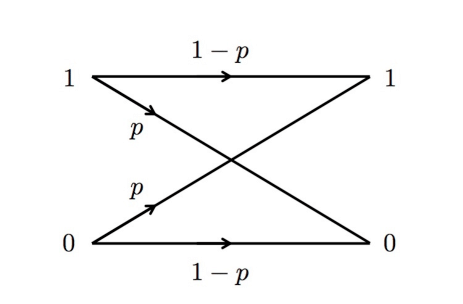
\includegraphics[width=\textwidth]{BSC.png}

We want to find channel capacity of this channel,

$$ C= \text{max}_{P_X} (I(X;Y))$$

\begin{align*}
    I(X;Y) &= H(Y) -H(Y/X) \\
    &= H(Y)- \sum_{x \in \{ 0, 1 \}} P_X(x) H(Y/X=x) \\
    &= H(Y)- \sum_{x \in \{ 0, 1 \}} P_X(x) H_2(p) \\
    &= H(Y) - H_2 (p)
\end{align*}

As we know $max(H(Y)) \leq Y$,

$$ C_{BSC} = 1- H_2(p)$$

where $H_2(p)$ is the binary entropy function defined by,
$$ H_2(x)= x \log_2 \frac{1}{x} + (1-x) \log_2 \frac{1}{1-x}$$

Hence if $P_x$ is a uniform distribution, the channel capacity can be 1.\\

We will now show the converse for the BSC(p) capacity. i.e. we will show that no matter what we do, we can't get a rate higher than $1- H_2 (p)$.

Let $C$ be the code which has rate close to capcity.
$$ R= \frac{ \log_2 |C|}{n} \Rightarrow |C| = 2^{nR}$$

Suppose $\underbar{c} \in C $ is transmitted, then
$$ C = (c_1, \cdots , c_n) \to \text{BSC(p)} \to (y_1, \cdots , y_n)$$

There are $\sim np$ positions in $\underbar{c}$ which are flipped to get $\mathcal{Y}$. (as the channel is independently acting on each bit)

We can expect any sequence in the set $S(\underbar{c})$ as the output sequence.
$$ S(\underbar{c})= \{ \mathcal{Y} \in \{0,1 \}^n : d_H (\underbar{c}, \mathcal{Y})= np\}$$

$d_H$ is the Hamming distance between $\mathcal{Y}$ \& $\underbar{c}$. i.e number of positions in $\underbar{c}$ which we have to flip.

Now around every codeword we draw this `Hamming ball' of radius $np$.

We want $S(\underbar{c1})$ and $S(\underbar{c2})$ to be close to empty to prevent many-one mapping.

Because the code $C$ has small probability of error, this means that the balls around the codewords in C are non-intersecting.

$$ \Rightarrow |C| \leq \frac{2^n}{|S(C)|}$$

$|S(C)|$ is the number of vectors in any ball and the same for any $\underbar{c} \in C = {n \choose np}$.
$$ \Rightarrow |C| \leq \frac{2^n}{{n \choose np}}$$
$$ \log_2 |C| \leq n- \log_2 {n \choose np} \leq n - n H_2 (p)$$
(as we have previously seen)

$$ \Rightarrow R= \frac{\log_2 |C|}{n} \leq 1- H_2 (p)$$
$$ \Rightarrow R \leq C_{BSC}$$

We have studied the result of Shannon's noisy coding channel theorem for the particular case of BSC. But Shannon's achievability result wasn't constructive (i.e. doesn't identify a code which works but rather shows the existence of one such code).

Such a class of channels is calles discrete memoryless channels (without feedback).

It took around 50 years to come up with candidate constructions which have rate close to capacity and small probability of error. This process is called coding theory.

\end{document}
